%\VignetteIndexEntry{Statistical Working Paper on balancing of the FBS}
%\VignetteEngine{knitr::knitr}

%\documentclass[nojss]{jss}
%\usepackage[]{graphicx}
%\usepackage[]{color}
%\usepackage{geometry}

\documentclass[nojss]{jss}\usepackage[]{graphicx}\usepackage[]{color}
%% maxwidth is the original width if it is less than linewidth
%% otherwise use linewidth (to make sure the graphics do not exceed the margin)
\makeatletter
\def\maxwidth{ %
  \ifdim\Gin@nat@width>\linewidth
    \linewidth
  \else
    \Gin@nat@width
  \fi
}
\makeatother

\definecolor{fgcolor}{rgb}{0.345, 0.345, 0.345}
\newcommand{\hlnum}[1]{\textcolor[rgb]{0.686,0.059,0.569}{#1}}%
\newcommand{\hlstr}[1]{\textcolor[rgb]{0.192,0.494,0.8}{#1}}%
\newcommand{\hlcom}[1]{\textcolor[rgb]{0.678,0.584,0.686}{\textit{#1}}}%
\newcommand{\hlopt}[1]{\textcolor[rgb]{0,0,0}{#1}}%
\newcommand{\hlstd}[1]{\textcolor[rgb]{0.345,0.345,0.345}{#1}}%
\newcommand{\hlkwa}[1]{\textcolor[rgb]{0.161,0.373,0.58}{\textbf{#1}}}%
\newcommand{\hlkwb}[1]{\textcolor[rgb]{0.69,0.353,0.396}{#1}}%
\newcommand{\hlkwc}[1]{\textcolor[rgb]{0.333,0.667,0.333}{#1}}%
\newcommand{\hlkwd}[1]{\textcolor[rgb]{0.737,0.353,0.396}{\textbf{#1}}}%

\usepackage{framed}
\makeatletter
\newenvironment{kframe}{%
 \def\at@end@of@kframe{}%
 \ifinner\ifhmode%
  \def\at@end@of@kframe{\end{minipage}}%
  \begin{minipage}{\columnwidth}%
 \fi\fi%
 \def\FrameCommand##1{\hskip\@totalleftmargin \hskip-\fboxsep
 \colorbox{shadecolor}{##1}\hskip-\fboxsep
     % There is no \\@totalrightmargin, so:
     \hskip-\linewidth \hskip-\@totalleftmargin \hskip\columnwidth}%
 \MakeFramed {\advance\hsize-\width
   \@totalleftmargin\z@ \linewidth\hsize
   \@setminipage}}%
 {\par\unskip\endMakeFramed%
 \at@end@of@kframe}
\makeatother

\definecolor{shadecolor}{rgb}{.97, .97, .97}
\definecolor{messagecolor}{rgb}{0, 0, 0}
\definecolor{warningcolor}{rgb}{1, 0, 1}
\definecolor{errorcolor}{rgb}{1, 0, 0}
\newenvironment{knitrout}{}{} % an empty environment to be redefined in TeX

\usepackage{alltt}
\usepackage{url}
\usepackage[sc]{mathpazo}
\usepackage{geometry}
\geometry{verbose,tmargin=2.5cm,bmargin=2.5cm,lmargin=2.5cm,rmargin=2.5cm}
\setcounter{secnumdepth}{2}
\setcounter{tocdepth}{2}
\usepackage{breakurl}
\usepackage{hyperref}
\usepackage[ruled, vlined]{algorithm2e}
\usepackage{mathtools}
%\usepackage{draftwatermark}
\usepackage{float}
\usepackage{placeins}
\usepackage{mathrsfs}
\usepackage{multirow}
\usepackage{courier}


%% maxwidth is the original width if it is less than linewidth
%% otherwise use linewidth (to make sure the graphics do not exceed the margin)
\makeatletter
\def\maxwidth{ %
  \ifdim\Gin@nat@width>\linewidth
    \linewidth
  \else
    \Gin@nat@width
  \fi
}
%\makeatotherx


%\usepackage{framed}
%\makeatletter
%\newenvironment{kframe}{%
% \def\at@end@of@kframe{}%
% \ifinner\ifhmode%
%  \def\at@end@of@kframe{\end{minipage}}%
%  \begin{minipage}{\columnwidth}%
% \fi\fi%
% \def\FrameCommand##1{\hskip\@totalleftmargin \hskip-\fboxsep
% \colorbox{shadecolor}{##1}\hskip-\fboxsep
%     % There is no \\@totalrightmargin, so:
%     \hskip-\linewidth \hskip-\@totalleftmargin \hskip\columnwidth}%
% \MakeFramed {\advance\hsize-\width
%   \@totalleftmargin\z@ \linewidth\hsize
%   \@setminipage}}%
% {\par\unskip\endMakeFramed%
% \at@end@of@kframe}
%\makeatother

%\definecolor{shadecolor}{rgb}{.97, .97, .97}
%\definecolor{messagecolor}{rgb}{0, 0, 0}
%\definecolor{warningcolor}{rgb}{1, 0, 1}
%\definecolor{errorcolor}{rgb}{1, 0, 0}
%\newenvironment{knitrout}{}{} % an empty environment to be redefined in TeX

\usepackage{alltt}
\usepackage{url}
\usepackage[sc]{mathpazo}
%\usepackage{geometry}
%\geometry{verbose,tmargin=2.5cm,bmargin=2.5cm,lmargin=2.5cm,rmargin=2.5cm}
\setcounter{secnumdepth}{2}
\setcounter{tocdepth}{2}
\usepackage{breakurl}
\usepackage{hyperref}
%\usepackage[ruled, vlined]{algorithm2e}
%\usepackage{mathtools}
%\usepackage{draftwatermark}
%\usepackage{float}
%\usepackage{placeins}
%\usepackage{mathrsfs}
%\usepackage{multirow}
%% \usepackage{mathbbm}
%\DeclareMathOperator{\sgn}{sgn}
%\DeclareMathOperator*{\argmax}{\arg\!\max}

\title{\bf faoswsTrade}

\author{Marco Garieri \\ Food and Agriculture Organization \\ of
  the United Nations}

\Plainauthor{M. Garieri}

\Plaintitle{faoswsTrade: Documentation}

\Shorttitle{faoswsTrade}

\Abstract{

\noindent
This vignette provides a detailed description of the trade modules.\\
This paper is dynamically generated on \today{} and is subject to
changes and updates. Version 1.
}

\Keywords{Agricultural Trade, Tariff Line, Eurostat, Mirroring}

\Address{
  Marco Garieri\\
  Economics and Social Statistics Division (ESS)\\
  Economic and Social Development Department (ES)\\
  Food and Agriculture Organization of the United Nations (FAO)\\
  Viale delle Terme di Caracalla 00153 Rome, Italy\\
  E-mail: \email{marco.garieri@fao.org}\\
  URL: \url{https://github.com/SWS-Methodology/faoswsTrade}
}
\IfFileExists{upquote.sty}{\usepackage{upquote}}{}
\IfFileExists{upquote.sty}{\usepackage{upquote}}{}
\begin{document}

\newpage


The trade module is divided in two submodules: {\tt complete\_tf\_cpc} and {\tt total\_trade\_CPC}. Each module is year specific. This means that, at the time being, the trade module run indipendently for each year. In order to run the {\tt total\_trade\_CPC}, the output of {\tt complete\_tf\_cpc} is needed.\\
All tables and graphs present in this documentation are just examples. More details on the data are given in the code.

\section{Complete tf cpc}

\subsection{Data}
Raw data are provided by the SWS Team (subunit of Team F) for both UNSD Tariffline and Eurostat Data. The data have been already prefiltered in the following way:
\begin{itemize}
\item [\bf{Eurostat}]
\begin{itemize}
\item code of reporter (reporter) just numeric (letters are not allowed)
\item code of partner (partner) just numeric (letters are not allowed)
\item code of CN8 (hs) just numeric (letters are not allowed)
\end{itemize}

\begin{knitrout}
\definecolor{shadecolor}{rgb}{0.969, 0.969, 0.969}\color{fgcolor}\begin{kframe}
\begin{verbatim}
##   reporter partner       hs flow year  value weight   qty    hs6
## 1       11      10 85193000    2 2009  83.96    2.2  1010 851930
## 2       11      10 85198121    1 2009  17.89    0.2  5023 851981
## 3       11      10 85198121    2 2009 243.69    7.3 13894 851981
## 4       11      10 85198125    1 2009   1.06    0.0     5 851981
## 5       11      10 85198125    2 2009  17.07    0.0   171 851981
## 6       11      10 85198131    1 2009   9.90    0.0   159 851981
\end{verbatim}
\end{kframe}
\end{knitrout}

\item [\bf{UNSD}]
\begin{itemize}
\item code of HS (comm) just numeric (letters are not allowed)
\end{itemize}
\end{itemize}
If any codes are still alphanumeric please ask team F to check, since this step is performed by them.\\
The module downloads only records of commodities of interest for Tariffline Data. The HS chapters are the following: 01, 02, 03, 04, 05, 06, 07, 08, 09, 10, 11, 12, 13, 14, 15, 16, 17, 18, 19, 20, 21, 22, 23, 24, 33, 35, 38, 40, 41, 42, 43, 50, 51, 52, 53. In the future, if other commotidy are of interest for the division, it is important to include additional chapter in the first step of the downloading. For Eurostat Data no filtering is applied.

\begin{knitrout}
\definecolor{shadecolor}{rgb}{0.969, 0.969, 0.969}\color{fgcolor}\begin{kframe}
\begin{verbatim}
##   reporter partner       hs flow year     value weight qty qunit    hs6
## 1       90     458     3303    1 2009  54.75252     NA  NA     1   3303
## 2      184      36 07121000    1 2009 634.93650     NA  NA     1 071210
## 3      184      36 09011200    1 2009 470.57794     NA  NA     1 090112
## 4      184     554 12100000    1 2009 544.94550     NA  NA     1 121000
## 5      184     504 21050020    1 2009 379.96200     NA  NA     1 210500
## 6       90      36     5203    1 2009  36.37752     NA  NA     1   5203
\end{verbatim}
\end{kframe}
\end{knitrout}



\subsection{Process}
\subsubsection{Mapping UNSD Tariffline and Eurostat data}
At this stage a standardization/mapping step is performed. The details are devided between UNSD Tariffline and Eurostat due to the nature of the differences among the two datasets.
\begin{itemize}
\item [\bf{UNSD Tariffline}]
\begin{enumerate}
\item UNSD Tariffline data reports area code with Tariffline M49 standard (which are different for official M49). The area code is converted in FAO country code using a specific convertion table provided by Team ENV. Area codes not mapping to any FAO country code or mapping to code 252 (which correpond not defined area) are separately saved and removed from further analyses.
\begin{knitrout}
\definecolor{shadecolor}{rgb}{0.969, 0.969, 0.969}\color{fgcolor}\begin{kframe}
\begin{verbatim}
##     m49 fao
## 164 270  75
## 26  280  79
## 294 716 181
## 241 634 179
## 38  471 252
## 106  51   1
\end{verbatim}
\end{kframe}
\end{knitrout}

\item Commodity codes are reported in HS codes ({\it Harmonized Commodity Description and Coding System}). The codes are converted in FCL (FAO Commodity List) codes. This step is performed using table incorporated in the SWS. In this step, all the mapping between HS and FCL code is stored. If a country is not included in the package of the mapping for that specific year, all the records for the reporting country are removed. All records without an FCL mapping are filtered out and saved in specific variables.
\begin{knitrout}
\definecolor{shadecolor}{rgb}{0.969, 0.969, 0.969}\color{fgcolor}\begin{kframe}
\begin{verbatim}
##    validyear area flow   fromcode     tocode  fcl
## 1         NA   81    2 0407001900 0407001900 1062
## 2         NA  154    2 2009291100 2009291100  510
## 3       2009  157    1 0714200090 0714200090  122
## 4         NA  211    1   20059910   20059910  472
## 5         NA   84    2   02073685   02073685 1075
## 6         NA  101    2  230610000  230619999  332
## 7         NA   13    2   19052000   19052999   22
## 8         NA  236    2 0204210000 0204210000  977
## 9         NA  134    1   04069019   04069019  904
## 10        NA    9    1   09012100   09012199  657
\end{verbatim}
\end{kframe}
\end{knitrout}


\item Information of the FCL units is added.
\begin{knitrout}
\definecolor{shadecolor}{rgb}{0.969, 0.969, 0.969}\color{fgcolor}\begin{kframe}
\begin{verbatim}
##   fcl fclunit
## 1  15      mt
## 2  16      mt
## 3  17      mt
## 4  18      mt
## 5  19      mt
## 6  20      mt
\end{verbatim}
\end{kframe}
\end{knitrout}

\item Just for UNSD Tariffline data convertion of units of measurements are applied to meet FAO standards, where all weights are reported in metric tonnes, animals in heads or 1000 heads and for some commodity just the value is provided.
\item The flow codes of re-Import (4) are recoded into Import (1) and codes of re-Export (3) to Export (2). This procedure is applied following UNSD standards:
\begin{quote}
\underline{Distinction between Exports and Re-exports / Imports and Re-imports}\\
Exports of a country can be distinguished as exports of domestic goods and exports of foreign goods. The second class is generally referred to as re-exports. The exports shown in our database contain both the exports of domestic and foreign goods. Re-exports are exports of foreign goods in the same state as previously imported; they are to be included in the country exports. It is recommended that they be recorded separately for analytical purposes. This may require the use of supplementary sources of information in order to determine the origin of re-exports, i.e., to determine that the goods in question are indeed re-exports rather than the export of goods that have acquired domestic origin through processing. Re-imports are goods imported in the same state as previously exported. They are included in the country imports. It is recommended that they be recorded separately for analytical purposes. This may require the use of supplementary sources of information in order to determine the origin of re-imports, i.e., to determine that the goods in question are indeed re-imports rather than the import of goods that have acquired foreign origin through processing. There are several reasons why an exported good might return to the country of origin. The exported good might be defective, the importer might have defaulted on payments or cancelled the order, the authorities might have imposed an import barrier, or demand or prices in the country of origin might have made it worthwhile to bring the good back.
\end{quote}
\end{enumerate}

\item [\bf{Eurostat}]
\begin{enumerate}
\item Eurostat classifies areas in their geonomenclature. The are code is converted in FAO country code using a specific convertion  table, stored in the SWS, provided by Team B/C.  Area codes not mapping to any FAO country code or mapping to code 252 (which correpond not defined area) is reported and the records for these area codes are removed.
\begin{knitrout}
\definecolor{shadecolor}{rgb}{0.969, 0.969, 0.969}\color{fgcolor}\begin{kframe}
\begin{verbatim}
##   ComM49 FAO         Name
## 1      1  68 France      
## 2      2  15 Belg.-Luxbg 
## 3      3 150 Netherlands 
## 4      4  79 Fr Germany  
## 5      5 106 Italy       
## 6      6 229 Utd. Kingdom
\end{verbatim}
\end{kframe}
\end{knitrout}

\item Commodity codes are reported in CN8 codes (Combined Nomenclature 8 digits). The codes are converted in FCL (FAO Commodity List) codes. This step is performed using the same package ({\tt hsfclmap}) as for UNSD Tariffline.
If a specific record has a CN8 code not mapping to any specific FCL code, then the record is reported and removed. If a country is not included in the package of the mapping for that specific year, all the records for the reporting country are removed.\\
Eurostat data are already provided in the correct units of measurements and do not need futher conversions. (No need of example, same as before).
\item Information of the FCL units is added. This step is straighforward since for Eurostat the units are already corrected. (No need of example, same as before).
\item Values are converted from EUR to USD using the table, stored in the SWS, with avarage currency for each year provided by Team B/C.
\begin{knitrout}
\definecolor{shadecolor}{rgb}{0.969, 0.969, 0.969}\color{fgcolor}\begin{kframe}
\begin{verbatim}
##   Year ExchangeRate
## 1 2000     0.924020
## 2 2001     0.892860
## 3 2002     0.946000
## 4 2003     1.131200
## 5 2004     1.243304
## 6 2005     1.245755
\end{verbatim}
\end{kframe}
\end{knitrout}

\end{enumerate}
\end{itemize}

\subsubsection{Unified Official Trade Flows Dataset}
UNSD Tariffline and Eurostat datasets are ready to be merged togheter. From UNSD Tariffline all the European countries are removed and the final tables has all the countries worldwide.

\subsubsection{Standardization, editing and outlier detection}
\begin{itemize}
\item {\bf Application of Notes} Perennial and yearly specific notes are mdb files provided by the Team B/C already saved in a R friendly dataset. The notes might be of different nature. They might be a multiplicative factor, or forcing a value. More information  about the notes can be provided by team B/C. The notes might be year specific or for all years (in this case reported as NA) and might refer to HS or/and FCL codes. This notes (or adjustments) were developed during the years and they are available from 1997 to 2013. Notes of 2014 are copied from notes in 2013, as a partial solution, but this need future work in the future.\\
Comparing results between the new and the old procedure showed that sometimes the discrepancies between the two results are due to the application of the notes.\\
Remark: at the time being, the notes with unspecified year and with application of a factor 1000 are removed, since in the previous years UNSD was reporting some data in tonnes, while now it reports all data in kg.\\
More details on how to read the notes can be given by team B/C.
\begin{knitrout}
\definecolor{shadecolor}{rgb}{0.969, 0.969, 0.969}\color{fgcolor}\begin{kframe}
\begin{verbatim}
##   year flow      hs  fcl partner weight  qty value special reporter
## 1 2012    1      NA   17      NA     10 <NA>  <NA>    <NA>        8
## 2 2005    2      NA 1168      NA    100 <NA>  <NA>    <NA>       11
## 3   NA   NA      NA  836      NA    0.6 <NA>  <NA>    <NA>       52
## 4 2013    4      NA  702     194    0.1 <NA>  <NA>    <NA>       13
## 5 2011    1      NA 1061      NA    0.1 <NA>  <NA>    <NA>       37
## 6 2013    2 9030000  671     231     10 <NA>  <NA>    <NA>       33
\end{verbatim}
\end{kframe}
\end{knitrout}


\item {\bf Unit Values computation} For each record having both quantity and value (thus excluding all commodity reported just as value), the unit of value ($u_v$) is computed as following:
\begin{equation}
u_v = \frac{qty}{value}
\end{equation}

\item {\bf Outlier Detection and Imputation} Based on the untis of measurementes we might have cases of outlier. The target variables are traded quantities so the outlier test on the unit values is a tool to correct quantity data. The outlier are calculated based on the distribution of the unit of value for the same country, year and flow at the HS level (tariffline level). The reason to identify the outlier at the HS level is due to the fact that, under the same FCL code, different commodity might fall (i.e. maize seed and seed). The outlier are detecting using the Tukey's procedure:
\begin{itemize}
\item The Tukey's five number summary are calculated: minimum (m), lower-hinge ($lh$), median ($med$), upper-hinge ($uh$) and maximum ($M$).
\item The coefficient for the outlier detection is set up as suggested by Tukey to 1.5 ($coef$).
\item For each value is calculated a specific distance from the lower or the upper-hinge in the following way:
\begin{equation}
\text{x is outlier if} \begin{cases}
    x < lh - coef * iqr, & \text{lower outlier},\\
    x > up + coef * iqr, & \text{upper outlier}.
  \end{cases}
\end{equation}
\end{itemize}
where $iqr$ is the interquartile range.\\

The traded quantieis outlier are then corrected using the corresponding value (which remain fixed) and dividing it by the median unit of value of that specific commodity, country, flow and year. In this way only few official quantity data are corrected.\\
Remark: in the module, one of the input parameter for the user is the oultlier coefficient By default this is set up to 1.5. More info regaring the outlier coefficient is given in the Future Work section.

\item {\bf Missing Quantities Detection and Imputation} For records in which the commodity has to be reported in quantity and the quantity is missing and the value is present, the corresponding quantity is imputed dividing the corresponding value by the median of the units of value of the corresponding commodity (HS level/country/flow/year)
\end{itemize}

\subsubsection{Mirroring and Balancing}
The module produce the list of non-reporting countries: these are the countries present as partners but absent as reporters. For this countries the mirroring routine is applied: the corrisponding trade of the non-reporting countries are extracted from the partners inverting the flows. The quantities are the same while the values are corrected by a factor of 12\% due to the CIF/FOB conversion. This need more work, details in the Future Work section.\\

\subsection{Flags}
Both records with imputation with outlier or mirroring imputation have a special flag:
\begin{itemize}
\item {\tt flagObservationStatus}: this flag is {\bf I}, which means imputed
\item {\tt flagMethod}: this flag is {\bf e}, which means estimated with a statistical algorithm.
\end{itemize}
For all the other records empty string flags are saved.\\
More information on the Flag is given in the Future Work section.

\subsection{Convertion to FAO SWS standards}
At this point the table is almost ready to be save in the SWS. Additional mapping and aggregation are necessary in order to respect the SWS standards:
\begin{itemize}
\item Conversion of FCL into CPC codes. This conversion is based on the table of conversion 2.1 expanded. If some FCL codes are not mapped into CPC ones, the corresponding records are filtered out. Since the mapping between FCL and CPC is one-to-one there is no aggregation at this point. The routine just add the corresponding CPC code.
\item Concersion from FAO country code to M49.
\item Each row of the final output must be or quantity or value specific, while so far the module keeps this information in one row. We therefore split this information in two separated rows.
\end{itemize}

The first submodule save the final output in the {\tt completed\_tf\_cpc\_m49} dataset, within the {\tt trade} domain.

\section{Total trade CPC}
This second submodule uses as input the output of the previous submodule. These two modules are separated because the two outputs are needed for different purposes, not only, the resulting matrices have different dimensions.\\
This module aggregates total trade flow by reporting country for partners countries to a single total trade for each unique CPC commodity code.\\
The module save the ouput into the dataset {\tt total\_trade\_cpc\_m49}, within the {\tt trade} domain.

\newpage
\section{Flow Chart Process}
\begin{center}\includegraphics[scale = 0.01]{"trade_1"}\end{center}
\newpage
\begin{center}\includegraphics[scale = 0.01]{"trade_1_bis"}\end{center}
%\begin{center}\includegraphics[width=20mm,scale=0.1]{"trade_3"}\end{center}
%\begin{center}\includegraphics[width=20mm,scale=0.1]{"trade_4"}\end{center}


\newpage
\section{Future work}

\subsection{Validation Steps}
This section represents the most high priority task for the trade module.\\
\subsubsection{Raw Data - Data content assessment}
\begin{itemize}
\item[Progress status] In the vignettes folder, a sample of pre-analysis is given, but not integrated in the main module (file name: {\tt preanalysis\_2009.Rmd}). The pre-analysis script calculate the total number of recordsfor both Eurostat and UNSD Tariffline datasets and the distribution of lenght of the commodty HS codes (for UNSD Tariffline) and CN8 for Eurostat is performed. For each country we report if data includes imports, exports, re-exports and re-imports at all possible lenght. All records with hs-lenght (for UNSD Tariffline) or CN8-lenght (for Eurostat) less than 6 are removed. The pre-analysis script produces a html file.
\item[Next activities] The pre-analyses of the assessment of the data has to be integrated in the module. The script is just a guide but improvements are needed (i.e. tables).
\end{itemize}

\subsubsection{Report and check of discarded elements after mapping}
\begin{itemize}
\item[Progress status] At the moment the module is saving the unsolved mapping records in a separated variable, but not reported anywhere.
\item[Next activities] Each mapping routine might produce some unsolved mapping. All unsolved mapping should be reported and possibly solved in the future.
\end{itemize}

\subsubsection{Destination Table}
\begin{itemize}
\item[Next activities] The {\tt complete\_tf\_cpc} module produces output for all the records passing all the routines and not filtered out. The module does not check if any commodity is missing. A possible solution would be to have a destination table with all the commodities of interest and the module should fill the destination table. In this way the output validation step should be achieved.
\end{itemize}


\subsection{Time Series Analysis}
\begin{itemize}
\item[Next activities] Upon availability of time-series data, a check of the CPC-based unit values accross the time series should be performed. Differentiation between errors in the order of magnitude on quantities and values (time series) and outliers (cross section). An additional submodule of imputation of missing data using time series analysis would be a solution.
\end{itemize}


\subsection{CIF/FOB}
\begin{itemize}
\item[Progress status] The CIF/FOB correction for mirroring is, at the time being, set up to 12\%. This has been suggested by team B/C.
\item[Next activities] Additional work might be done in order to assess if the estimate is appropriate. There might be different range of percentages for different type of countries and by distance between reporters and partners. A study can be conducted on available records on both side: this means records for which the commodity is reported by the reporter and by the partner.
\end{itemize}

\subsection{Re-import and Re-export}
\begin{itemize}
\item[Progress status] All re-import and re-export is considered as, respectively, import and export.
\item[Next activities] More study might be conducted in order to identify countries more prone to report re-import and re-export.
\end{itemize}

\subsection{Self Trade Analysis}
\begin{itemize}
\item[Progress status] A script within the {\tt vignette} folder, named {\tt selftrade.R}, has been used to perform some simple analyses on the self trade. The script filter all records for which the reporter and the partner are the same. The script compute the sum of all value across all commodities per country (Figure 1), or the sum of all the value for each commodity across all countries (Figure 2). In this way we can spot out the countries reporting massive self trade as well as which are the main commodities reported in self trade.\\
This is an example of the graphical output (still part of the script).
\begin{center}
\begin{figure}
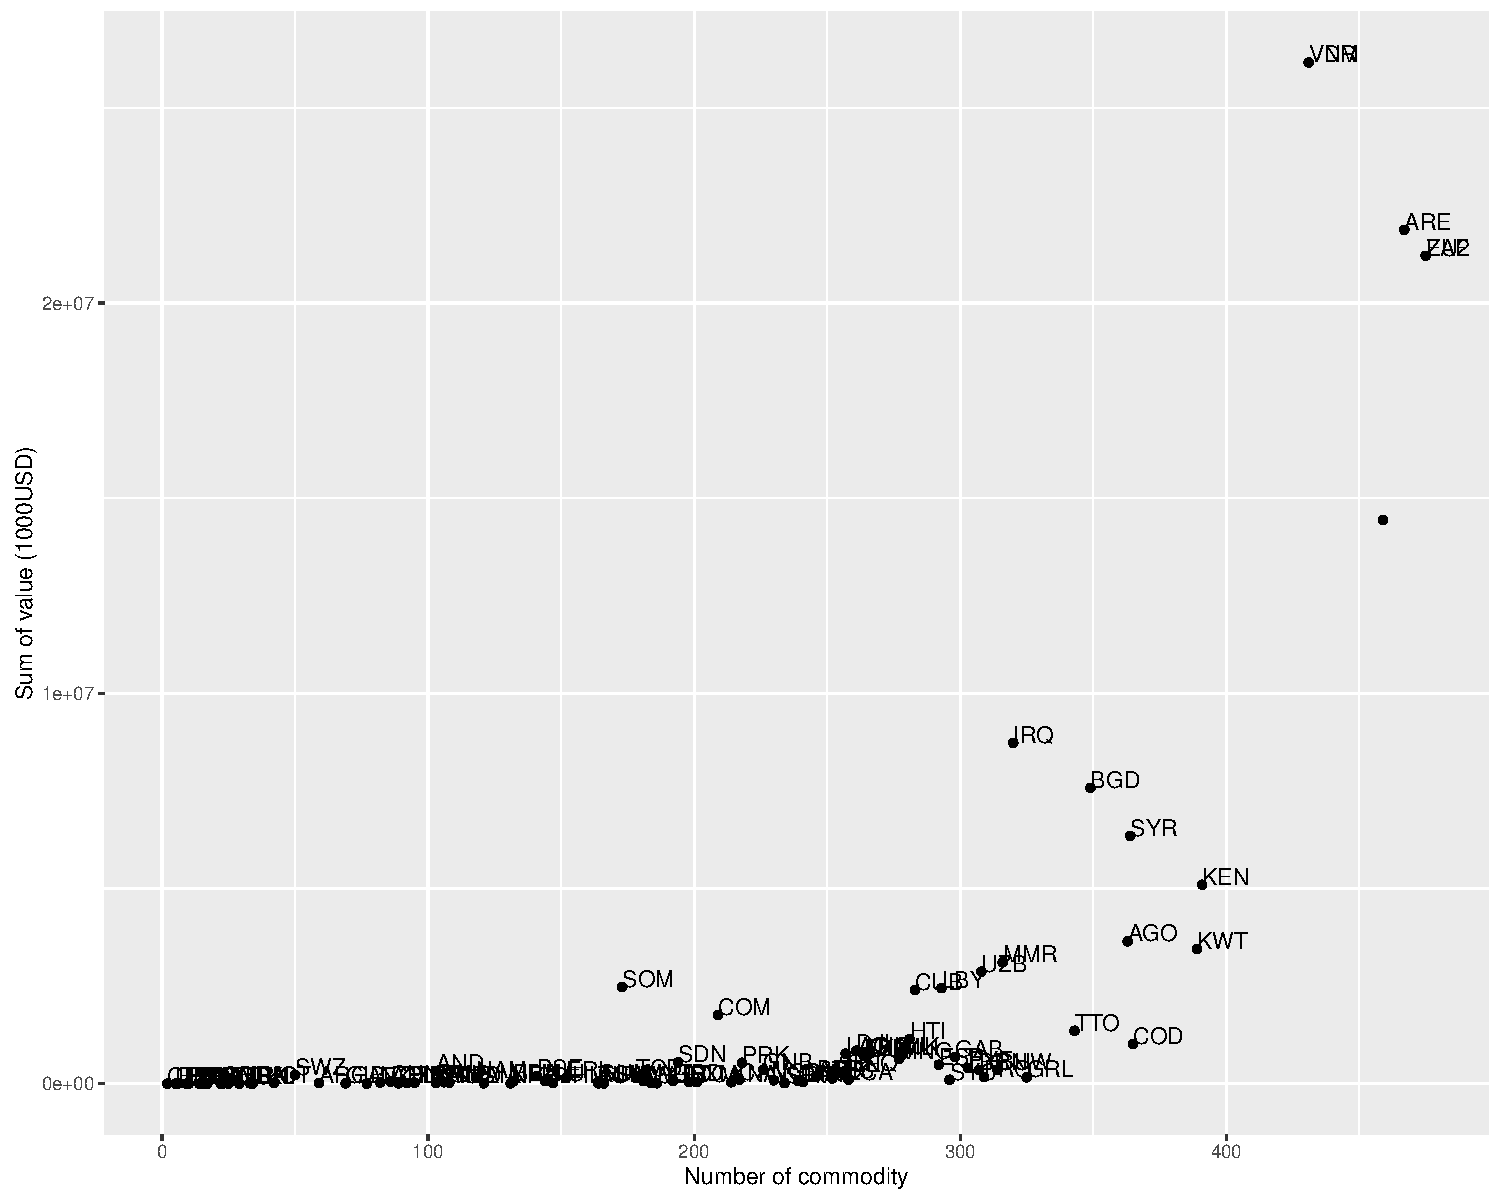
\includegraphics[scale=0.5]{../selftrade_by_country_name}
\caption{Sum of all self trade records by country.}
\end{figure}
\end{center}

\begin{center}
\begin{figure}
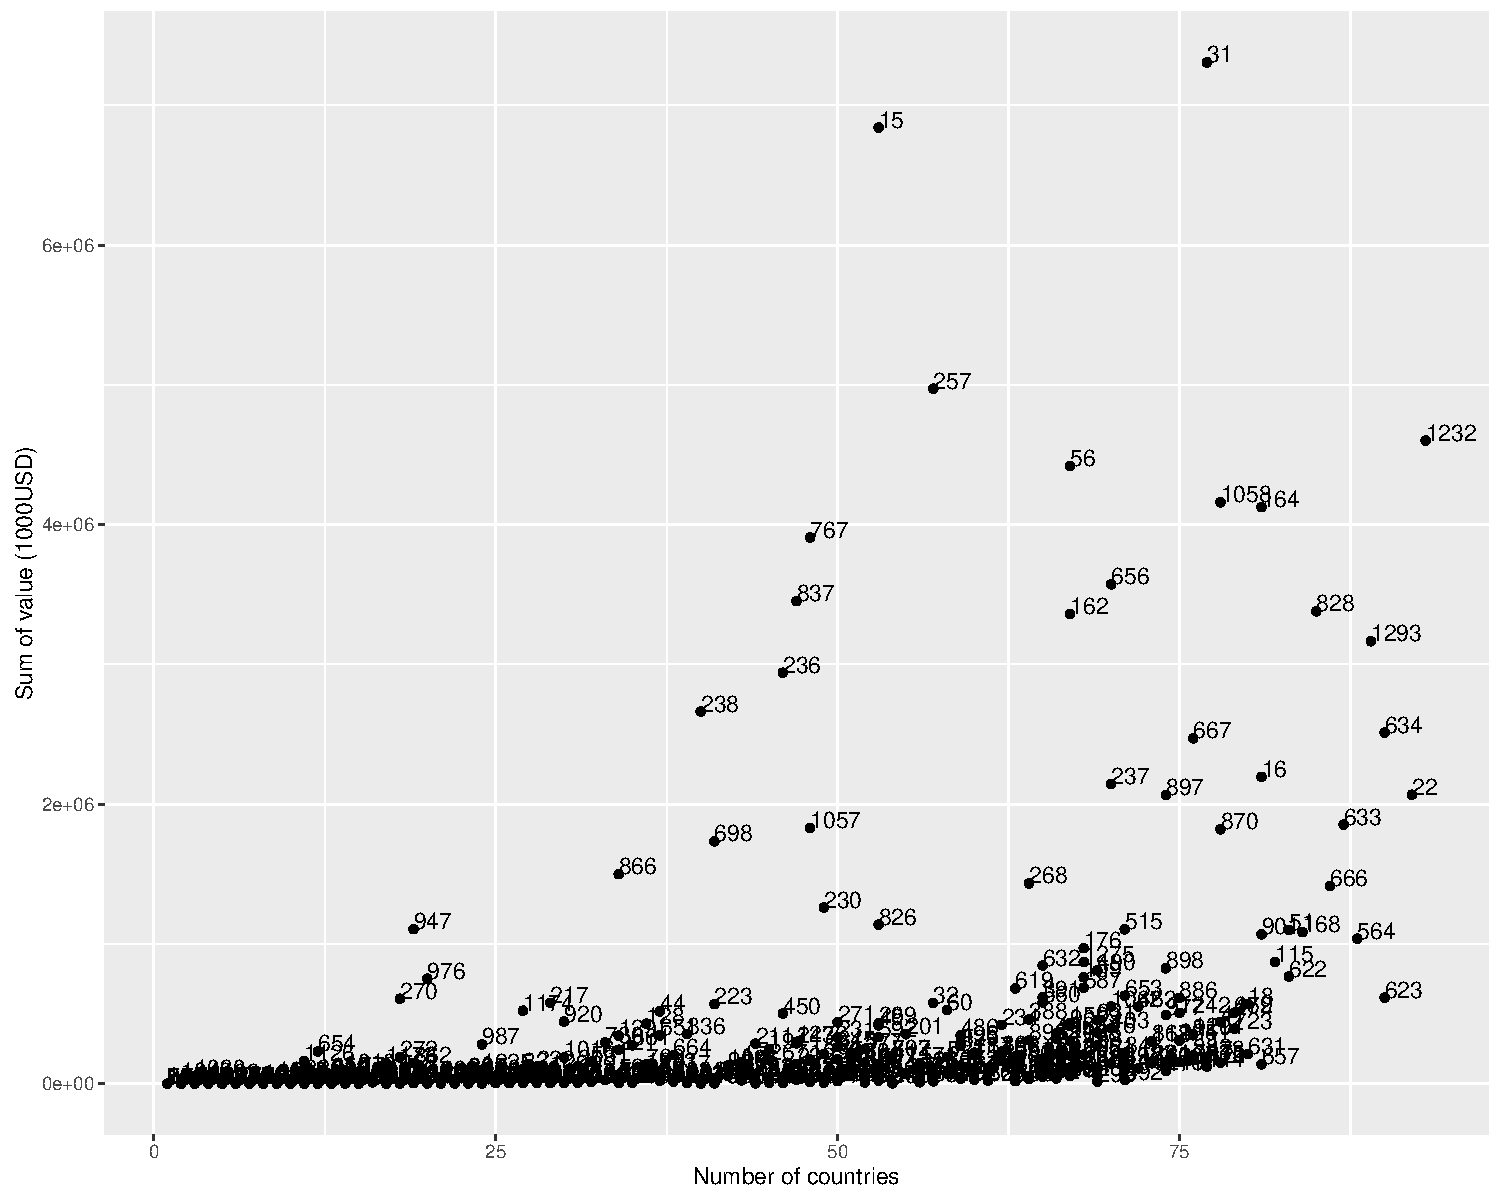
\includegraphics[scale=0.5]{../selftrade_by_commodity_code}
\caption{Sum of all self trade records by commodity. Codes in FCL.}
\end{figure}
\end{center}


\item[Next activities] This might be incorporated in the module and might produce suitable output within the SWS. More documentation is needed.
\end{itemize}

\subsection{Pseudo-automatic mapping of commodities}
\begin{itemize}
\item[Next activities] An additional method has to be added in the future: the algorithm should try to trim the code not mapped and try to map them with shorter HS codes. If any of shorter codes (from right to left) are then not mapped, we can definitely discard the record.
If a specific record has a HS code not mapping to any specific FCL code, then the record is reported and removed.
\end{itemize}

\subsection{Mapping from HS to FCL}
\begin{itemize}
\item[Progress status] In the module for commodities we have 2 different mapping. From HS to FCL, using mapping produced by team B/C and then from FCL to CPC 2.1. This mapping is available for the following years: 1997, 2001, 2002, 2003, 2004, 2005, 2006, 2007, 2008, 2009, 2010, 2011, 2012, 2013. The following years are missing: 1998, 1999, 2000. The mapping for 2014 has been copied from year 2013, but the results need to be checked.
\item[Next activities] In the future direct mapping from HS to CPC has been asked from managment. A possible solution, where adding the column with the one-to-one CPC codes has been sent to Carola (09.06.2016), but anyway this needs revision (\href{https://drive.google.com/drive/folders/0B_Z6srBtmyJRUmtaaXphTllZUDA}{link})
\end{itemize}

\subsection{Mapping from Comtrade M49 and Geonomenclature directly to M49}
\begin{itemize}
\item[Progress status] The country codes, as the commodity ones, have two step of mapping. This results in higher risk of data loss due to unsolved mapping.
\item[Next activities] A direct map from Comtrade M49 (Tariffline UNSD) to M49 and from Geonomenclature (Eurostat) to M49 would be ideal.
\end{itemize}

\subsection{Flag correction}
\begin{itemize}
\item[Pending activities] This activities have high priority
\begin{enumerate}
\item When mirroring is performed, the quantity will stay official, while the value will change flag (high priority)
\item In case of official figure the methodology has to be 'h' and not empty.
\end{enumerate}
\end{itemize}

\subsection{Outlier coefficient}
\begin{itemize}
\item[Progress status] The outlier coefficient is set up to 1.5. The outlier coefficient is a input parameter of the {\tt complete\_tf\_cpc} submodule.
\item[Pending activities] After discussion with team B/C (23.06.2016) a specific analysis has to be perfomed to understand what is the best coefficient to be used in order to reflect old results. After this analysis, the outlier coefficient should be hard-coded within the code of the module without letting the user to modify it anymore.
\end{itemize}


\subsection{Food-aid}
\begin{itemize}
\item[Next activities] This has to be incorporated also to understand the trend in a time series analysis. This needs special study to understand if we can get the data just from the exports not reported as imports in the partner.
\end{itemize}

\section*{Disclaimer}
This Working Paper should not be reported as representing the official view of
the FAO. The views expressed in this Working Paper are those of the
author and do not necessarily represent those of the FAO or FAO
policy. Working Papers describe research in progress by the authors and
are published to elicit comments and to further discussion.\\




\end{document}
Status API Training Shop Blog About
ÔøΩ 2015 GitHub, Inc. Terms Privacy Security Contact
%
